\documentclass[a4paper,12pt]{article}
\usepackage{fullpage} % Package to use full page
\usepackage[utf8]{inputenc}
%\setlength\parindent{0pt}
\usepackage{amsmath} %for writing text in equations with \text{}
\usepackage{dsfont} %for identity matrix
\usepackage[T1]{fontenc}
\usepackage{slashed}
\usepackage{tikz}
\usepackage{gensymb}
\usepackage{wrapfig}

\newcommand{\icol}[1]{% inline column vector
  \left(\begin{smallmatrix}#1\end{smallmatrix}\right)%
}

\newcommand{\irow}[1]{% inline row vector
  \begin{smallmatrix}(#1)\end{smallmatrix}%
}

\title{\textbf{Gauge Theories: Electroweak}}
\author{Lecturer: Richard Ball}
\date{\normalsize\today} % Can't work out how to make this a UK format but oh well

\begin{document}

\maketitle
\section{Introduction}
%
Imagine a world without electroweak:
\begin{itemize}
    \item Still have electromagnetism (EM), massive hadrons, atoms, gravity etc.
    \item Parity (P) and charge conjugation (C) are still good symmetries
    \item Flavour is always conserved: everything lasts forever (and always existed)
    \item No neutrinos (would be non-interacting)
\end{itemize}
%
Neutrinos were first hypothesised by Pauli (1930) to explain the missing energy in $\beta$-decay. They were first observed in 1956 (Cowan-Reines). Parity violation was first directly observed in 1956/7 (Lee-Yang-Wu).

\subsection{Chirality}
%
Define the projection operators $P_R \equiv \frac{1}{2}(1 + \gamma^5)$ and $P_L \equiv \frac{1}{2}(1 - \gamma^5)$. Recalling that $(\gamma^5)^2 = 1$ and $(\gamma^5)^\dagger = \gamma^5$, we can deduce the following properties:
\begin{itemize}
    \item $P_R^2 = P_R$
    \item $P_L^2 = P_L$
    \item $P_LP_R = P_RP_L = 0$
    \item $P_R + P_L = 1$
    \item $P_R - P_L = \gamma^5$.
\end{itemize}
% 
Any Dirac spinor can be split up into a right-handed and a left-handed component, $\psi = \psi_R + \psi_L$, using the projection operators to define $\psi_R = P_R \psi$ and $\psi_L = P_L \psi$. Since $\gamma^\mu P_L = P_R \gamma^\mu$, it follows that $\bar{\psi} P_R \equiv (\bar{\psi})_R = \bar{\psi}_L$ and $\bar{\psi} P_L \equiv (\bar{\psi})_L = \bar{\psi}_R$. So 
\begin{equation}
\begin{split}
    \bar{\psi}\psi = \bar{\psi}(\psi_R + \psi_L) &= \bar{\psi}_L\psi_R + \bar{\psi}_R\psi_L \\
    &\text{and} \\
    \bar{\psi}\gamma^\mu \psi = \bar{\psi}\gamma^\mu(\psi_R + \psi_L) &= \bar{\psi}_R\gamma^\mu\psi_R 
    \bar{\psi}_L\gamma^\mu\psi_L.
\end{split}
\end{equation}
%
The Dirac Lagrangian splits up like 
\begin{equation}
\begin{split}
\mathcal{L}_D &= \bar{\psi}(i\slashed{\partial}-m)\psi \\ 
&= \bar{\psi}_R i\slashed{\partial}\psi_R + \bar{\psi}_L i\slashed{\partial}\psi_L
+ m(\bar{\psi}_L\psi_R + \bar{\psi_R}\psi_L)
\end{split}
\end{equation}
so the mass term mixes $\psi_R$ and $\psi_L$: if $m \to 0$, $\psi_R$ and $\psi_L$ are independent. In this scenario they are both 2-component spinors obeying the Weyl equation $i\slashed{\partial}\psi_{R/L} = 0$.

\subsection{Helicity}
The spin operator can be expressed as $\Sigma^i = \frac{i}{2} \epsilon^{ijk}[\gamma^j, \gamma^k] = \gamma^5\gamma^0\gamma^i$. Then $[P_L, \Sigma^i] = [P_R, \Sigma^i]$: spin and chirality commute. Now consider \textit{helicity}, defined 
\begin{equation}
    h \equiv \frac{2\underline{\Sigma} \cdot \underline{p}}{|\underline{p}|}.
\end{equation}
$h$ has eigenvalues $\pm1$, which follows from $(\slashed{p} - m)u^\pm = 0 \implies hu^\pm = \pm u^\pm$. But $\slashed{p} = E\gamma^0 - \underline{\gamma}\cdot\underline{p}$ and $h = \gamma^5\gamma^0 (\underline{\gamma}\cdot\underline{p})/|\underline{p}| = \gamma^5\gamma^0(E\gamma^0 - \slashed{p})$. So
%
\begin{equation}
\begin{split}
\gamma^5(E - \gamma^0\slashed{p})u^\pm &= \pm u^\pm \\
\implies (P_R-P_L)(E-\gamma^0m)u^\pm &= \pm p(P_R + P_L)u^\pm \\
\text{ and } (E \mp p)u_R^\pm &= m\gamma^0 u_L^\pm \\
             (E \pm p)u_L^\pm &= m\gamma^0 u_R^\pm. 
\end{split}
\end{equation}
Again, the mass term mixes R and L, but if $m \to 0$, $p = E + \mathcal{O}(\frac{m^2}{E})$ and $2E u_R^- = 2E u_L^+ = 0$ so $u_R^- = u_L^+ = 0$, i.e. $u_R$ has helicity +1 and $u_L$ has helicity -1. 

Note that when $m=0$, helicity is Lorentz invariant (no rest frame). For $m \neq 0$, 
\begin{equation}
\begin{split}
    u_R^- = \frac{m\gamma^0}{E+p}u_L^- &\approx \frac{m}{2E}\gamma^0u_L^- \\
    \text{ and } u_L^+ &\approx \frac{m}{2E}\gamma^0u_R^+.
\end{split}
\end{equation}
You get similar expressions for negative energy solutions:
\begin{equation}
\begin{split}
\text{for $m = 0$:   } &v_R^- = v_L^+ = 0 \\
\text{for $m \neq 0$:    }  &v_R^- = -\frac{m\gamma^0}{2E}v_L^- \text{ and } v_L^+ = -\frac{m\gamma^0}{2E}v_R^-.
\end{split}
\end{equation}
%
\subsection{The Chiral Representation}
%
In the chiral representation the gamma matrices can be expressed as:
\[ \gamma^0 = \left( \begin{array}{cc}
0 & 1  \\
1 & 0  \end{array} \right) \qquad
\gamma^i = \left( \begin{array}{cc}
0 & -\sigma^i  \\
\sigma^i & 0  \end{array} \right) \qquad
\gamma^5 = \left( \begin{array}{cc}
1 & 0 \\
0 & -1     \end{array} \right)\] 
%
so
%
\[ P_R = \left( \begin{array}{cc}
1 & 0  \\
0 & 0  \end{array} \right) \qquad
P_L = \left( \begin{array}{cc}
0 & 0  \\
0 & 1  \end{array} \right) \qquad
\implies
\psi = \left( \begin{array}{c}
\psi_R  \\
\psi_L      \end{array} \right).\] 
%
Furthermore, the spin operator can be written
%
\[ \Sigma^i = \gamma^5\gamma^0\gamma^i = \left( \begin{array}{cc}
\sigma^i & 0  \\
0 & \sigma^i  \end{array} \right) \]
%
so the helicity eigenstates are $\icol{\psi_R^\pm\\0}$ and $\icol{0\\\psi_L^\pm}$. Now consider the positive and negative energy solutions. 
%
$(\slashed{p} - m)u =0 \implies$
%
\[ \left( \begin{array}{cc}
-m & E +\underline{\sigma}\cdot\underline{p}  \\
  E -\underline{\sigma}\cdot\underline{p}& -m  \end{array} \right)
\left( \begin{array}{c}
u_R   \\
u_L  \end{array} \right) = 0.\] 
%
But $\underline{\sigma}\cdot \underline{p}\ u_{L/R} = \pm p\ u_{L/R}^\pm$ so $(E \pm p)u_L^\pm = m\ u_R^\pm$. Using $E^2 = p^2 + m^2$:
\begin{equation}
\begin{split}
(E \pm p)u_L^\pm &= \sqrt{(E+p)(E-p)}u_R^\pm \\
\implies \sqrt{E\pm p}\ u_L^\pm &= \sqrt{E \mp p}\ u_R^\pm 
\end{split}
\end{equation}
and we can write
%
\[ u^\pm =
\left( \begin{array}{c}
\sqrt{E \pm p} \ \xi^\pm   \\
\sqrt{E \mp p} \ \xi^\pm  \end{array} \right) \] 
%
where $\xi^+ = \icol{1\\0}$ and $\xi^- = \icol{0\\1}$. 
\newline
\newline
\textit{Exercise: check that the normalisations $\bar{u}u = 2m$, $u^\dagger u = 2E$.}
\newline

Similarly, $(\slashed{p} +m)v = 0$ and $(\underline{\sigma}\cdot\underline{p})v^\pm = \mp p\ v^\pm$, so 
\begin{equation}
\begin{split}
(E \mp p)v_L^\pm &= -m\ v_R^\pm \\
\implies \sqrt{E\mp p}\ v_L^\pm &= -\sqrt{E \pm p}\ v_R^\pm 
\end{split}
\end{equation}
and
%
\[ v^\pm =
\left( \begin{array}{c}
\sqrt{E \mp p} \ \xi^\pm   \\
-\sqrt{E \pm p} \ \xi^\pm  \end{array} \right). \] 
%
You can relate $\xi^\pm$ to $\chi^\pm$ by charge conjugation: $v^\pm = i \gamma^2 u^{\pm *}$, where
%
\[ i\gamma^2 = \left( \begin{array}{cc}
0 & -i \sigma^2  \\
i\sigma^2 & 0  \end{array} \right); \qquad 
-i\sigma^2 = \left( \begin{array}{cc}
0 & -1 \\
1 & 0 \end{array} \right) \]
%
so $\chi^\pm = -i\sigma^2\xi^\pm$ and if $\xi^\pm = \icol{1\\0}, \icol{0\\1}$ then $\chi^\pm = \icol{0\\1}, \icol{-1\\0}$ as before.
%
\subsection{Parity}
%
Under P, $\psi \to \psi_p = \gamma^0\psi$. We know that $P_L \gamma^0 = \gamma^0 P_R$, so $\psi_L \to \gamma^0 \psi_L =  P_R\gamma^0 \psi_L = (\psi_p)_R$. In other words, $(\psi_L)_p = (\psi_p)_R$, so parity switches L and R.

Note that $[\gamma^0, \Sigma^i] = 0$ but under P $\underline{p} \to - \underline{p}$ so $h \to -h$, as expected. This means $u_R^+ to u_L^-$ etc.: parity flips helicity but not spin.
%
\subsection{Charge conjugation}
%
Under C, $\psi \to \psi_c = C\overline{\psi}^T$ where $C = i\gamma^2\gamma^0$. Then $P_LC = CP_L$ so $\psi_L \to C(\overline{\psi})_L^T$. 
This means that charge conjugation leaves the chirality unchanged. Helicity is also unchanged: C just takes particles $\leftrightarrow$ antiparticles.
%
\subsection{Time reversal}
%
Under T, $\psi \to \psi_T = B\psi$ where $B = i\gamma^1\gamma^3 = -i\gamma^5C$ and $B^\dagger = B = B^{-1}$. Again, $P_LB = BP_L$ so $\psi_L \to B\psi_L$ and time reversal leaves chirality and helicity unchanged (it reverses both spin and momentum). 
%
%%%%%%%%%%%%%%%%%%%%%%%%%%%%%%%%%%%%%%%%%%%%%%%%%%%%%%%%%%%%%%%%%%%%%%%%%%%%%%%%%%%%%%%%%%%%%%%%%%%%%%%%%
%
\section{Charged Current Electroweak}
%
\subsection{Fermi Theory (1934)}
%
Fermi theory is based on a point-like 4-fermion interaction
\begin{equation}
    G_F(\bar{n}\gamma_\mu p)(\bar{\nu}\gamma^\mu e)
\end{equation}
representing the process $n \to pe^-\bar{\nu}$, where $n$ is a neutron, $p$ is a proton, $e^-$ is an electron and $\bar{\nu}$ is an antineutrino. More generally, the interaction can be written as $G_F J_\mu^\dagger J^\mu$ where $J_\mu$ is the "weak current" and is composed of leptonic and hadronic contributions: $J_\mu = \bar{\nu}\gamma_\mu e + \bar{p}\gamma_\mu n + ...$. Note that $J_\mu$ has $\Delta Q = +1$ so $J_\mu^\dagger$ has $\Delta Q = -1$ and electric charge is conserved. 

Considering mass dimensions $[\cdot]$: $[m\psi\bar{\psi}]=+\psi$, $[\psi]=3/2$ and $[J_\mu] =3$ so $[G_F]=-2$. In other words, the coupling scales as 1/mass$^2$. The mass scale is $\approx$ 300 GeV, so the interaction is weak. The original Fermi interaction conserves parity (and C and CP), just like QED. This turned out to be wrong, according to theory developed by Lee and Yang (1956) and the Wu experiment in 1957. In weak interactions, P and C are violated by CP is conserved. More on this later.
%
\subsection{V-A Theory}
%
Developed by Masshart, Sudarshan, Feynman, Gell-Man ... in 1958. V-A theory is based on a vector current $V_\mu$ and an axial current $A_\mu$,
\begin{equation}
\begin{split}
V_\mu &= \bar{\nu}\gamma_\mu e + \bar{p}\gamma_\mu n + ... \\
A_\mu &= \bar{\nu}\gamma_\mu \gamma^5 e + \bar{p}\gamma_\mu \gamma^5 n + ...
\end{split}
\end{equation}
whose difference gives the overall current
\begin{equation}
\begin{split}
\frac{1}{2}J_\mu = \frac{1}{2}(V_\mu - A_\mu)  &= \bar{\nu}\gamma_\mu\frac{1}{2}(1-\gamma^5) e + \bar{p}\gamma_\mu\frac{1}{2}(1-\gamma^5) n + ... \\
&= \bar{\nu}_L\gamma_\mu e_L + \bar{p}_L\gamma_\mu n_L + ... .
\end{split}
\end{equation}
So the weak interactions involve \textbf{only left-handed fields}, and maximally violate P and C. In fact, under P, C and CP the currents transform in the following ways:
\begin{equation}
\begin{split}
&P \qquad V^\mu \to V_\mu, \qquad A^\mu \to -A_\mu, \qquad (V-A)^\mu \to (V+A)_\mu \\
&C \qquad V^\mu \to -V^\mu, \qquad A^\mu \to A^\mu, \qquad (V-A)^\mu \to (-V-A)^\mu \\
&CP \qquad V^\mu \to -V_\mu, \qquad A^\mu \to -A_\mu, \qquad (V-A)^\mu \to -(V-A)_\mu 
\end{split}
\end{equation}
so $(V-A)^{\mu \dagger}(V-A)_\mu$ is invariant under CP (and T). 

Note that that neutrinos \textbf{only} interact weakly, so $\nu_R$ does not interact at all! If neutrinos are massless, there is no need for $\nu_R$. From 1930-1998 neutrinos were always assumed to be massless: here we will assume $m_\nu=0$ so $\nu$ are always left handed and $\bar{\nu}$ are always right handed. In reality $m_\nu \leq$ 0.3 eV, which is very small.

So we have
%
\begin{equation}
\mathcal{L}_{4F} = -\frac{G_F}{\sqrt{2}} J_\mu^\dagger J^\mu
\end{equation}
where the $\sqrt{2}$ is historical. $J_\mu = J_\mu^l + J_\mu^h$ can be split up into a leptonic and a hadronic current, each of which comprises three generations. For example, the leptonic current
\begin{equation}
\frac{1}{2}J_\mu^l = \bar{\nu}_e\gamma_\mu e_L + \bar{nu}_{(\mu)}\gamma_\mu \mu_L + \bar{\nu}_\tau \gamma_\mu \tau_L.
\end{equation}
Lepton number $L_e = N_{e^-} - N_{e^+} - N_{\nu_e} + N_{\bar{\nu}_e}$ and the corresponding $L_\mu$ and $L_\tau$ are conserved, according to Noether's Theorem.  

The hadronic current
\begin{equation}
\frac{1}{2}J_\mu^h = \bar{u}_L\gamma_\mu d_L^\prime + \bar{c}_L \gamma_\mu s_L^\prime + \bar{t}_L \gamma_\mu b_L^\prime
\end{equation}
is simplest to express in terms of the quarks. The baryon number $B = \sum_{gen} (N_u -N_{\bar{u}} - N_d + N_{\bar{d}})$ is conserved. Things are complicated due to the effects of quark mixing - see later.

(V-A) Theory is quite complicated, but there is only one coupling, $G_F$: we call this universality. Explicitly,
\begin{equation}
\mathcal{L}_{4F} = -\frac{G_F}{\sqrt{2}} (J_\mu^{l \dagger} J^{l\mu} + (J_\mu^{h \dagger} J^{l\mu} + J_\mu^{l \dagger} J^{h\mu}) + J_\mu^{h \dagger} J^{h\mu} ) 
\end{equation}
so there are three types of (charged current) weak interaction
\begin{itemize}
    \item \textbf{leptonic:} only leptons (and neutrinos) e.g. $\mu \to e \nu_\mu \bar{\nu}_e$
    \item \textbf{semi-leptonic:} both leptons and quarks e.g. $\pi^- = d\bar{u} \to \mu^- \bar{\nu}_\mu$
    \item \textbf{hadronic:} only quarks e.g. $\Lambda \to p \pi$
\end{itemize}
But all of them violate P and C and conserve CP, only involve left-handed particles and only involve one coupling $G_F$. 
\newline
\newline
\textbf{Example:} $\pi^+ \approx u\bar{d} \to \mu^+ \nu_\mu$. 
\newline
Fig. \ref{pioncp} demonstrates the sequential application of C and P to this process. Neither of the intermediate steps can happen, as they involve either a right-handed neutrino or a left-handed antineutrino.
\begin{figure}[h!]
\caption{Visualisation of applying C and P to the process $\pi^+ \approx u\bar{d} \to \mu^+ \nu_\mu$.}
\label{pioncp}
\centering
\begin{tikzpicture}
\draw[<-] (0,1) -- (1,1);
\node[] at (0,0.5) {$\mu^-$};
\draw[fill=black] (1.5,1) circle (0.1cm);
\node[] at (1.5,0.5) {$\pi^-$};
\draw[->] (2,1) -- (3,1) ;
\node[] at (3, 0.5){$\bar{\nu}_\mu$};
%
\draw[<-] (-4,3) -- (-3,3);
\node[] at (-4,2.5) {$\mu^+$};
\draw[fill=black] (-2.5,3) circle (0.1cm);
\node[] at (-2.5,2.5) {$\pi^+$};
\draw[->] (-2,3) -- (-1,3) ;
\node[] at (-1, 2.5){$\nu_\mu$};
%
\draw[->] (5.5,3) -- (6.5,3);
\node[] at (6.5,2.5) {$\mu^-$};
\draw[fill=black] (5,3) circle (0.1cm);
\node[] at (5,2.5) {$\pi^-$};
\draw[->] (4.5,3) -- (3.5,3) ;
\node[] at (3.5, 2.5){$\bar{\nu}_\mu$};
%
\draw[<-] (0,6) -- (1,6);
\node[] at (0,5.5) {$\nu_\mu$};
\draw[fill=black] (1.5,6) circle (0.1cm);
\node[] at (1.5,5.5) {$\pi^-$};
\draw[->] (2,6) -- (3,6) ;
\node[] at (3, 5.5){$\mu^+$};
%
\draw[->] (1.5,5) --(1.5,2) ;
\draw[->] (2.5,5) --(4.5,4) ;
\draw[->] (0.5,5) --(-1.5,4) ;
\draw[<-] (2.5,1.5) --(4.5,2) ;
\draw[<-] (0.5,1.5) --(-1.5,2) ;
%
\node[] at (2,3.5) {CP};
\node[] at (4,5) {C};
\node[] at (-1,5) {P};
\node[] at (-1,1.5) {C};
\node[] at (4,1.5) {P};
%
\draw[red,->] (2.5,1.25) -- (3,1.25);
\draw[red,->] (0,6.25) -- (0.5,6.25);
\draw[red,->] (-1.5,3.25) -- (-1,3.25);
\draw[red,->] (3.5,3.25) -- (4,3.25);
\end{tikzpicture}
\end{figure}
%
\subsection{Leptonic decays}
%
\textbf{Example:} $\mu^- \to e^- \bar{\nu}_e \nu_\mu$. 
\newline

\begin{wrapfigure}{l}{0.4\linewidth}
  \centering
  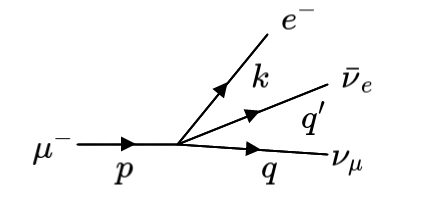
\includegraphics[width=\linewidth]{figs/diag_1.png}
\end{wrapfigure}
We will work with Dirac spinors everywhere and contract the spiniors as required.
The matrix element can be written
\begin{equation}
  \mathcal{M} = \langle e^-(k);\bar{\nu}_e(q^\prime)|\mathcal{L}_{4F}|\mu^-(p) \rangle
\end{equation}
and we can identify the Feynman rule for the four fermion vertex as 
\begin{equation}
  -i\frac{G_F}{\sqrt{2}} [\gamma_\mu(1-\gamma^5)]_{ab} [\gamma^\mu(1-\gamma^5)]_{cd}
\end{equation}
so 
\begin{equation}
  \mathcal{M} = -i\frac{G_F}{\sqrt{2}} \bigg(\bar{u}(k)\gamma^\mu(1-\gamma^5)v(q^\prime)\bigg) \bigg(\bar{u}(q)\gamma_\mu(1-\gamma^5)u(p)\bigg)
\end{equation}
where $\bar{u}(k)$, $v(q^\prime)$, $\bar{u}(q)$ and $u(p)$ refer to the electron, anti-electron neutrino, muon neutrino and muon respectively. 

Average over initial spins and sum over final spins (assuming the neutrinos are massless):
\begin{equation}
    \frac{1}{2} \sum_{spins} |\mathcal{M}|^2 = \frac{1}{4}G_F^2\ tr\bigg((\slashed{k}+m_e)\gamma^\mu(1-\gamma^5)\slashed{q}^\prime\gamma^\nu(1-\gamma^5)\bigg)\ tr\bigg(\slashed{q}\gamma_\mu(1-\gamma^5)(\slashed{p}+m_\mu)\gamma_\nu(1-\gamma^5)\bigg)
\end{equation}
where we call the first trace $\mathcal{M}^{\mu \nu}(k,q^\prime)$ and the second trace $\mathcal{M}_{\mu \nu}(q,p)$. Consider evaluating one of these traces, using $(1-\gamma^5)^2 = 2(1-\gamma^5)$ and $tr\gamma^5\gamma^\mu \gamma^\nu \gamma^\alpha \gamma^\beta = 4i\epsilon^{\mu \nu \alpha \beta}$:
\begin{equation}
\begin{split}
    \mathcal{M}_{\mu \nu}(q,p) &= 2\ tr\bigg( \slashed{q}\gamma_\mu(\slashed{p} + m_\mu)\gamma_\nu(1-\gamma^5)\bigg)\\
    &= 8(q_\mu p_\nu + p_\mu q_\nu - \eta_{\mu \nu} p \cdot q - i \epsilon_{\alpha \mu \beta \nu} q^\alpha p^\beta) \\
    &= 8(q_\mu p_\nu + p_\mu q_\nu - \eta_{\mu \nu} p \cdot q + i \epsilon_{\mu \nu \alpha \beta} q^\alpha p^\beta) 
\end{split}
\end{equation}
so
\begin{equation}
\begin{split}
\frac{1}{2}\sum_{spins}|\mathcal{M}|^2 &= 16\ G_F^2(k^\mu q^{\prime \nu} + q^{\prime \mu} k^\nu - \eta^{\mu \nu} k \cdot q^\prime - i \epsilon^{\mu \nu \alpha \beta} q^{\prime \alpha} k_\beta)(q_\mu p_\nu + p_\mu q_\nu - \eta_{\mu \nu} p \cdot q + i \epsilon_{\mu \nu \rho \sigma} q^\rho p^\sigma) \\
&= 16\ G_F^2(2p\cdot k q \cdot q^\prime + 2 p \cdot q^\prime k \cdot q + 4 p \cdot q k \cdot q^\prime - 4 k \cdot q^\prime p \cdot q + \epsilon^{\mu \nu \alpha \beta} \epsilon_{\mu \nu \rho \sigma} q^\prime_\alpha k_\beta q^\rho p^\sigma) \\
&= 64\ G_F^2 p \cdot q^\prime k \cdot q.
\end{split}
\end{equation}
Now we want to evaluate the decay rate in the lab frame of the muon. Here $E(p) = m_\mu$.
\begin{equation}
\begin{split}
d\Gamma &= \frac{1}{2m_\mu}\frac{1}{2}\sum_{spins}|\mathcal{M}|^2(dPS)_3 \\
& = \frac{1}{2m_\mu} \int \frac{d^3k}{(2\pi)^3 2k^0}\frac{d^3q}{(2\pi)^3 2q^0}\frac{d^3q^\prime}{(2\pi)^3 2q^{\prime 0}}(2\pi)^4\delta^4(p-k-q-q^\prime)\frac{1}{2}\sum_{spins}|\mathcal{M}|^2 \\
&= \frac{G_F^2}{8 m_\mu \pi^5} \int \frac{d^3k}{k^0} \frac{d^3q}{q^0} \frac{d^3q^\prime}{q^{\prime 0}} \delta^4(p-k-q-q^\prime)(p \cdot q^\prime)(k \cdot q).
\end{split}
\end{equation}
Integrate over $q$ and $q^\prime$, since these are unobserved. Write $Q = q + q^\prime = p - k$, $Q^2 = 2 q \cdot q^\prime = 2(q^0 q^{\prime 0} -\underline{q}\cdot \underline{q}^\prime) \geq 0$. Then we need to evaluate the integral
\begin{equation}
	\mathcal{I}_{\mu \nu}(Q) \equiv \int \frac{d^3q}{q^0} \frac{d^3 q^\prime}{q^{\prime 0}} \delta^4(Q - q - q^\prime) q_\mu q^\prime_\nu.
\end{equation}
Appealing to Lorentz invariance, we can write $\mathcal{I}_{\mu \nu} = a Q_\mu Q_\nu + b \eta_{\mu \nu} Q^2$ for some $a$, $b$ to be found. This is because these are the only two Lorentz invariant terms which can be constructed using the vectors and tensors available. In order to find the coefficients $a$ and $b$, we can systematically contract the expression with $\eta^{\mu \nu}$ and $Q^\mu Q^\nu$. This gives
\begin{equation}
\begin{split}
a + 4b &= \frac{1}{2}\mathcal{I} \\
a + b &= \frac{1}{4}\mathcal{I} \\
\text{where } \mathcal{I} &= \int \frac{d^3q}{|q|} \frac{d^3 q^\prime}{|q^\prime|} \delta^4(Q - q - q^\prime).
\end{split}
\end{equation}
and we have used $q^0 = |q|$, $Q \cdot q Q \cdot q^\prime = (q \cdot q^\prime)^2 = 1/4\ Q^4$. Since $\mathcal{I}$ is a Lorentz scalar, we can evaluate it in any frame. Choose $Q^\mu = (Q^0, \underline{0})$, where $\underline{q} = - \underline{q^\prime}$.
\begin{equation}
\begin{split}
\mathcal{I} &= \int \frac{d^3\underline{q}}{|\underline{q}|^2}\ \delta(Q^0 - 2 |\underline{q}|) \\
&= 4 \pi \int_0^\infty dq\ \delta(Q^0 - 2q) \\
&= 2 \pi
\end{split}
\end{equation}
so $a = \pi /3$ and $b= \pi /6$. Putting everything together,
\begin{equation}
p^\mu k^\nu \mathcal{I}_{\mu \nu}(Q) = \frac{1}{6} \pi (2 Q \cdot p Q \cdot k + p \cdot k Q^2)
\end{equation}
so 
\begin{equation}
\begin{split}
    d\Gamma &= \frac{G_F^2}{3 m_\mu (2\pi)^4)} \int \frac{d^3\underline{k}}{k^0}\ \bigg(2p \cdot (p-k) k \cdot (p-k) + p \cdot k (p-k)^2\bigg) \\
    &= \frac{G_F^2}{3 m_\mu (2\pi)^4)}  \int \frac{d^3\underline{k}}{k^0}\ \bigg(-2p^2k^2 + 3(p^2+k^2)p \cdot k -4(p \cdot k)^2\bigg)
\end{split}
\end{equation}
In the muon rest frame, $p \cdot k = m_\mu E$, where $E \equiv k^0$, and $\frac{d^3\underline{k}}{k^0} \to 4\pi |\underline{k}|dE$. We can ignore $m_e \ll m_\mu$. Then
\begin{equation}
    d\Gamma = \frac{2G_F^2}{3(2\pi)^3} m_\mu E^2(3m_\mu - 4E)dE
\end{equation}
but $Q^2 > 0$ so $m_\mu^2 - 2p\cdot k = m_\mu(m_\mu - 2e) >0$, i.e. $E < m_\mu/2$. The total cross-section
\begin{equation}
\begin{split}
    \Gamma &= \frac{G_F^2}{12\pi^3} m_\mu \int_0^{m_\mu/2} dE (3m_\mu E^2 - 4E^3) \\
    &= \frac{G_F^2 m_\mu^5}{192 \pi^3}.
\end{split}
\end{equation}
We can then use this to determine $G_F$: $\tau_\mu$ = 2.2$\times 10^{-6}$s and $\Gamma_\mu$ = 3.0$\times 10^{-19}$GeV, so $G_F \approx 1.2\times 10^{-5}$GeV$^{-2}$. 

You can use the same expression for $\tau^- \to \mu^- \bar{\nu}_\mu \nu_\tau$, $e^- \bar{\nu}_e \nu_\tau$ as a nice test of universality: $\Gamma(\tau^- \to \mu^- \bar{\nu}_\mu \nu_\tau) = \Gamma(\tau^- \to e^- \bar{\nu}_e \nu_\tau) = B\ \Gamma_\tau = (\frac{m_\tau}{m_\mu})^5\ \Gamma_\mu \approx 4 \times 10^{-13}$GeV.

\subsection{Semi-leptonic decays}
\textbf{Example: } $\pi^+ \to \mu^+ \nu_\mu$.
\newline

\begin{wrapfigure}{l}{0.4\linewidth}
  \centering
  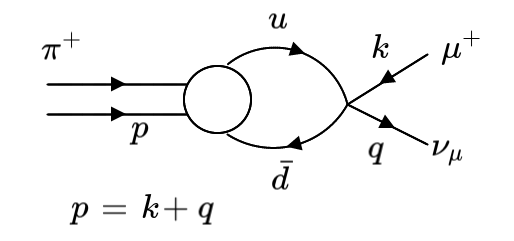
\includegraphics[width=\linewidth]{figs/diag_2.png}
\end{wrapfigure}
The matrix element can be written 
\begin{equation}
\begin{split}
    \mathcal{M} &= \langle \mu^+(k) \nu_\mu(q) | \mathcal{L}_{4F} | \pi^+(p) \rangle \\
    &= \frac{-iG_F}{\sqrt{2}} \bar{u}(q)\gamma^\mu(1-\gamma^5)v(k) \langle 0 | \bar{d}\gamma_\mu(1-\gamma^5)u | \pi^+(p) \rangle
\end{split}
\end{equation}
in other words, it factorises into a lepton piece and a quark piece, where the quark piece is of $V_\mu - A_\mu$ form. The pion is a pseudoscalar, so $\langle 0 | V_\mu | \pi^+ \rangle = 0$. The $\langle 0 | A_\mu | \pi^+ \rangle$ piece is a four-vector, so Lorentz invariance means it must take the form $\langle 0 | A_\mu | \pi^+ \rangle = i f_\pi p_\mu$, with $f_\mu$ some "pion decay constant" to be found. This means we can write
\begin{equation}
    \mathcal{M} = \frac{G_F f_\pi}{\sqrt{2}}\bar{u}(q)\slashed{p}(1-\gamma^5)v(k).
\end{equation}
But $p = k + q$, and using $\slashed{q}u(q)=0$; $(\slashed{k} + m_\mu)v(k)=0$ gives $\bar{u}(q)(\slashed{k} + \slashed{q})(1-\gamma^5)v(k) = -m_\mu \bar{u}(q)(1+ \gamma^5) v(k)$. Now we would like to evaluate the spin-averaged matrix element squared, taking note that $(1+\gamma^5)m_\mu(1-\gamma^5)=0$:
\begin{equation}
\begin{split}
\sum_{spins}|\mathcal{M}|^2 &= \frac{G_F^2}{2} f_\pi^2 m_\mu^2 tr\ \slashed{q}(1+\gamma^5) \slashed{k} (1-\gamma^5) \\
&= 4G_F^2 f_\pi^2 m_\mu^2\ k \cdot q \\
&= 2G_F^2 f_\pi^2 m_\mu^2(m_\pi^2 - m_\mu^2).
\end{split}
\end{equation}
In the lab frame,
\begin{equation}
    d\Gamma = \frac{1}{2m_\mu} \sum_{spins} |\mathcal{M}|^2(dPS)_2
\end{equation}
while
\begin{equation}
\begin{split}
\int(dPS)_2 &= \frac{1}{(4\pi)^2} \frac{|\underline{k}|}{m_\pi} \int d\Omega \\
&= \frac{1}{4\pi}\frac{|\underline{k}|}{m_\pi}
\end{split}
\end{equation}
where $|\underline{k}| = (m_\pi^2 - m_\mu^2)/2m_\pi$, so
\begin{equation}
\Gamma = \frac{1}{8\pi} G_F^2f_\pi^2 \frac{m_\mu^2}{m_\pi^3}(m_\pi^2 - m_\mu^2)^2.
\end{equation}
Using the measured rate for $\tau = 2.6 \times 10^{-8}$s, we can calculate $f_\pi \approx 130$ MeV. Note that 
\begin{equation}
\frac{\Gamma(\pi \to e \nu_e)}{\Gamma(\pi \to \mu \nu_\mu)} = \frac{m_e^2}{m_\mu^2}\frac{(m_\pi^2 - m_e^2)}{(m_\pi^2 - m_\mu^2)} \approx 10^{-4}.
\end{equation}
This is a good test of lepton universality. The ratio vanishes as $m_e \to 0$: this is because of helicity conservation. 
%
\subsection{Cabibbo mixing (1963)}
The Kaon decay $K^+ (u\bar{s}) \to \mu^+ \nu_\mu$ works similarly: $\langle 0 | A_\mu | K^+(p) \rangle = i f_k p_\mu$, and from experiment
\begin{equation}
    \frac{\Gamma(K \to \mu\nu)}{\Gamma(\pi \to \mu\nu)} \approx 1.3. 
\end{equation}
But if $\mathcal{L}_{4F}$ contained $\bar{u}_L \gamma_\mu s_L$ (in an analogy with $\bar{u}_L \gamma_\mu d_L$) we expect
\begin{equation}
    \frac{\Gamma(K \to \mu\nu)}{\Gamma(\pi \to \mu\nu)} = \frac{f_K^2}{f_\pi^2}\frac{m_\pi^3}{m_K^3}\frac{(m_K^2 - m_\mu^2)^2}{(m\pi^2 - m_\mu^2)^2} \approx 24
\end{equation}
since $f_K/f_\pi \approx 1.2$, i.e. SU(3) symmetry breaking is small.

The explanation is down to the form of the hadronic weak current. In actual fact this is
\begin{equation}
 \frac{1}{2}J_\mu^h = \bar{u}_L\gamma_\mu(\cos\theta_c\ d_L + \sin\theta_c\ s_L) + ... 
\end{equation}
where the term in brackets can be thought of as $d_L^\prime$, a \textit{mixture} of $d$ and $s$. Then 
\begin{equation}
    \Gamma(\pi \to \mu\nu) = \frac{G_F^2}{4\pi} f_\pi^2 \frac{m_\mu^2}{m_\pi^3}(m_\pi^2 - m_\mu^2)^2 \cos^2\theta_c
\end{equation} 
and
\begin{equation}
    \Gamma(K \to \mu\nu) = \frac{G_F^2}{4\pi} f_K^2 \frac{m_\mu^2}{m_K^3}(m_K^2 - m_\mu^2)^2 \sin^2\theta_c.
\end{equation} 
The Cabibbo angle, $\theta_c \approx 13\degree$, so $\cos\theta_c = 0.97$ and $\sin\theta_c = 0.22$. This reduces the relative size of $\Gamma(K \to \mu\nu)$ by a factor of roughly 20. We will revisit quark mixing later - stay tuned!
%
\subsection{Beta decay}
$n \to p\ e^- \bar{\nu}_e$.
\newline

\begin{wrapfigure}{l}{0.4\linewidth}
  \centering
  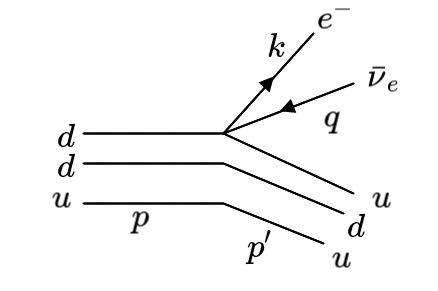
\includegraphics[width=\linewidth]{figs/diag_3.png}
\end{wrapfigure}
What's really going on is $d \to u\ e^- \bar{\nu}_e$: the other quarks are "spectators". Again, the matrix element factorises:
\begin{equation}
\begin{split}
    \mathcal{M} &= \langle p(p^\prime) e^-(k)\bar{\nu}_e(q) | \mathcal{L}_{4F} | n(p) \rangle \\
    &= \frac{-iG_F}{\sqrt{2}} \bar{u}(k)\gamma^\mu(1-\gamma^5)v(q)\\
    &\times \langle p(p^\prime) | \bar{d}^\prime\gamma_\mu(1-\gamma^5)u | n(p) \rangle \cos\theta_c.
\end{split}
\end{equation}
Considering the hadronic part,
\begin{equation}
\langle p(p^\prime) | (V_\mu - A_\mu) | n(p) \rangle = \cos\theta_c\bar{u}(p^\prime)\gamma_\mu(g_v-g_A\gamma^5)u(p)
\end{equation}
where $g_V =1$ and $g_A = 1.25$. Then 
\begin{equation}
\begin{split}
\frac{1}{2}\sum_{spins}|\mathcal{M}|^2 &= \frac{1}{4}G_F^2\cos^2\theta_c\ tr\bigg((\slashed{k} + m_e)\gamma^\mu(1-\gamma^5)\slashed{q}\gamma^\mu(1-\gamma^5)\bigg)\\
&\times tr\bigg((\slashed{p}^\prime + m_p) \gamma_\mu(1-g_A\gamma^5)(\slashed{p}+m_n)\gamma_\nu(1-g_A\gamma^5)\bigg) \\
&= \frac{1}{4}G_F^2\cos^2\theta_c\ \mathcal{M}^{\mu\nu}(k,q)\tilde{\mathcal{M}}_{\mu\nu}(p^\prime,p).
\end{split}
\end{equation}
Recalling the previous calculation for $\mu \to e\ \nu \bar{\nu}$, 
\begin{equation}
\tilde{\mathcal{M}}_{\mu\nu}(p^\prime,p) = 4\bigg((p_\mu^\prime p_\nu + p_\mu p_\nu^\prime - \eta_{\mu\nu} p \cdot p^\prime)(1+g_A^2) + i g_A \epsilon_{\mu\nu\alpha\beta}p^{\prime \alpha}p^\beta + m_n m_p(1-g_A^2)\eta_{\mu\nu}\bigg)
\end{equation}
so
\begin{equation}
\begin{split}
\frac{1}{2}\sum_{spins}|\mathcal{M}|^2 &= 8 G_F^2\cos^2\theta_c\ \bigg((2p\cdot k p^\prime \cdot q + 2 p\cdot q p^\prime \cdot k)(1+g_A)^2 \\
&- 4g_A(k\cdot p q\cdot p^\prime - k\cdot p^\prime q\cdot p) - 2 m_n m_p(1-g_A^2)k \cdot q\bigg)\\
&= 16G_F^2\cos^2\theta_c\ \bigg(p\cdot k p^\prime \cdot q (1-g_A)^2 + p\cdot q p^\prime \cdot k (1+ g_A)^2 - m_n m_p k \cdot q \bigg).
\end{split}
\end{equation}
The decay rate
\begin{equation}
\begin{split}
d\Gamma &= \frac{1}{2m_n} \int\frac{d^3k}{(2\pi)^32k^0} \int\frac{d^3q}{(2\pi)^32q^0} \int\frac{d^3p^\prime}{(2\pi)^32p^{\prime 0}}\ (2\pi)^4 \delta^4(p - p^\prime -k - q)\frac{1}{2}\sum_{spins}|\mathcal{M}|^2 \\
&= \frac{1}{16m_n(2\pi)^5}\int\frac{d^3k}{k^0} \int\frac{d^3q}{q^0}\frac{1}{p^{\prime 0}}\ \delta(p^0 - p^{\prime 0} - k^0 - q^0) \frac{1}{2}\sum_{spins}|\mathcal{M}|^2.
\end{split}
\end{equation}
Now write $p^0 = E_p$, $p^{\prime 0} = E_p$, $k^0 = E_e$, $q^0 = E_\nu$ and $d^3k = p_e E_e\ dE_e\ d\Omega_e$, $d^3q = E_\nu^2\ dE_\nu\ d\Omega_\nu$. Using $p_e^2 = E_e^2 - m_e^2$ we can rewrite $p_e\ dp_e = E_e\ dE_e$. So

\end{document}
